	\begin{figure}
	    	\captionsetup{width=\columnwidth}
	   	\centering
	   	\includegraphics[width=\columnwidth]{./graphics/errorAbs.png}
	   	\caption{Measured errors of state transition model and observation models.}
		\label{fig:err1}
	\end{figure}
	
	\begin{figure}
	    	\captionsetup{width=\columnwidth}
	   	\centering
	   	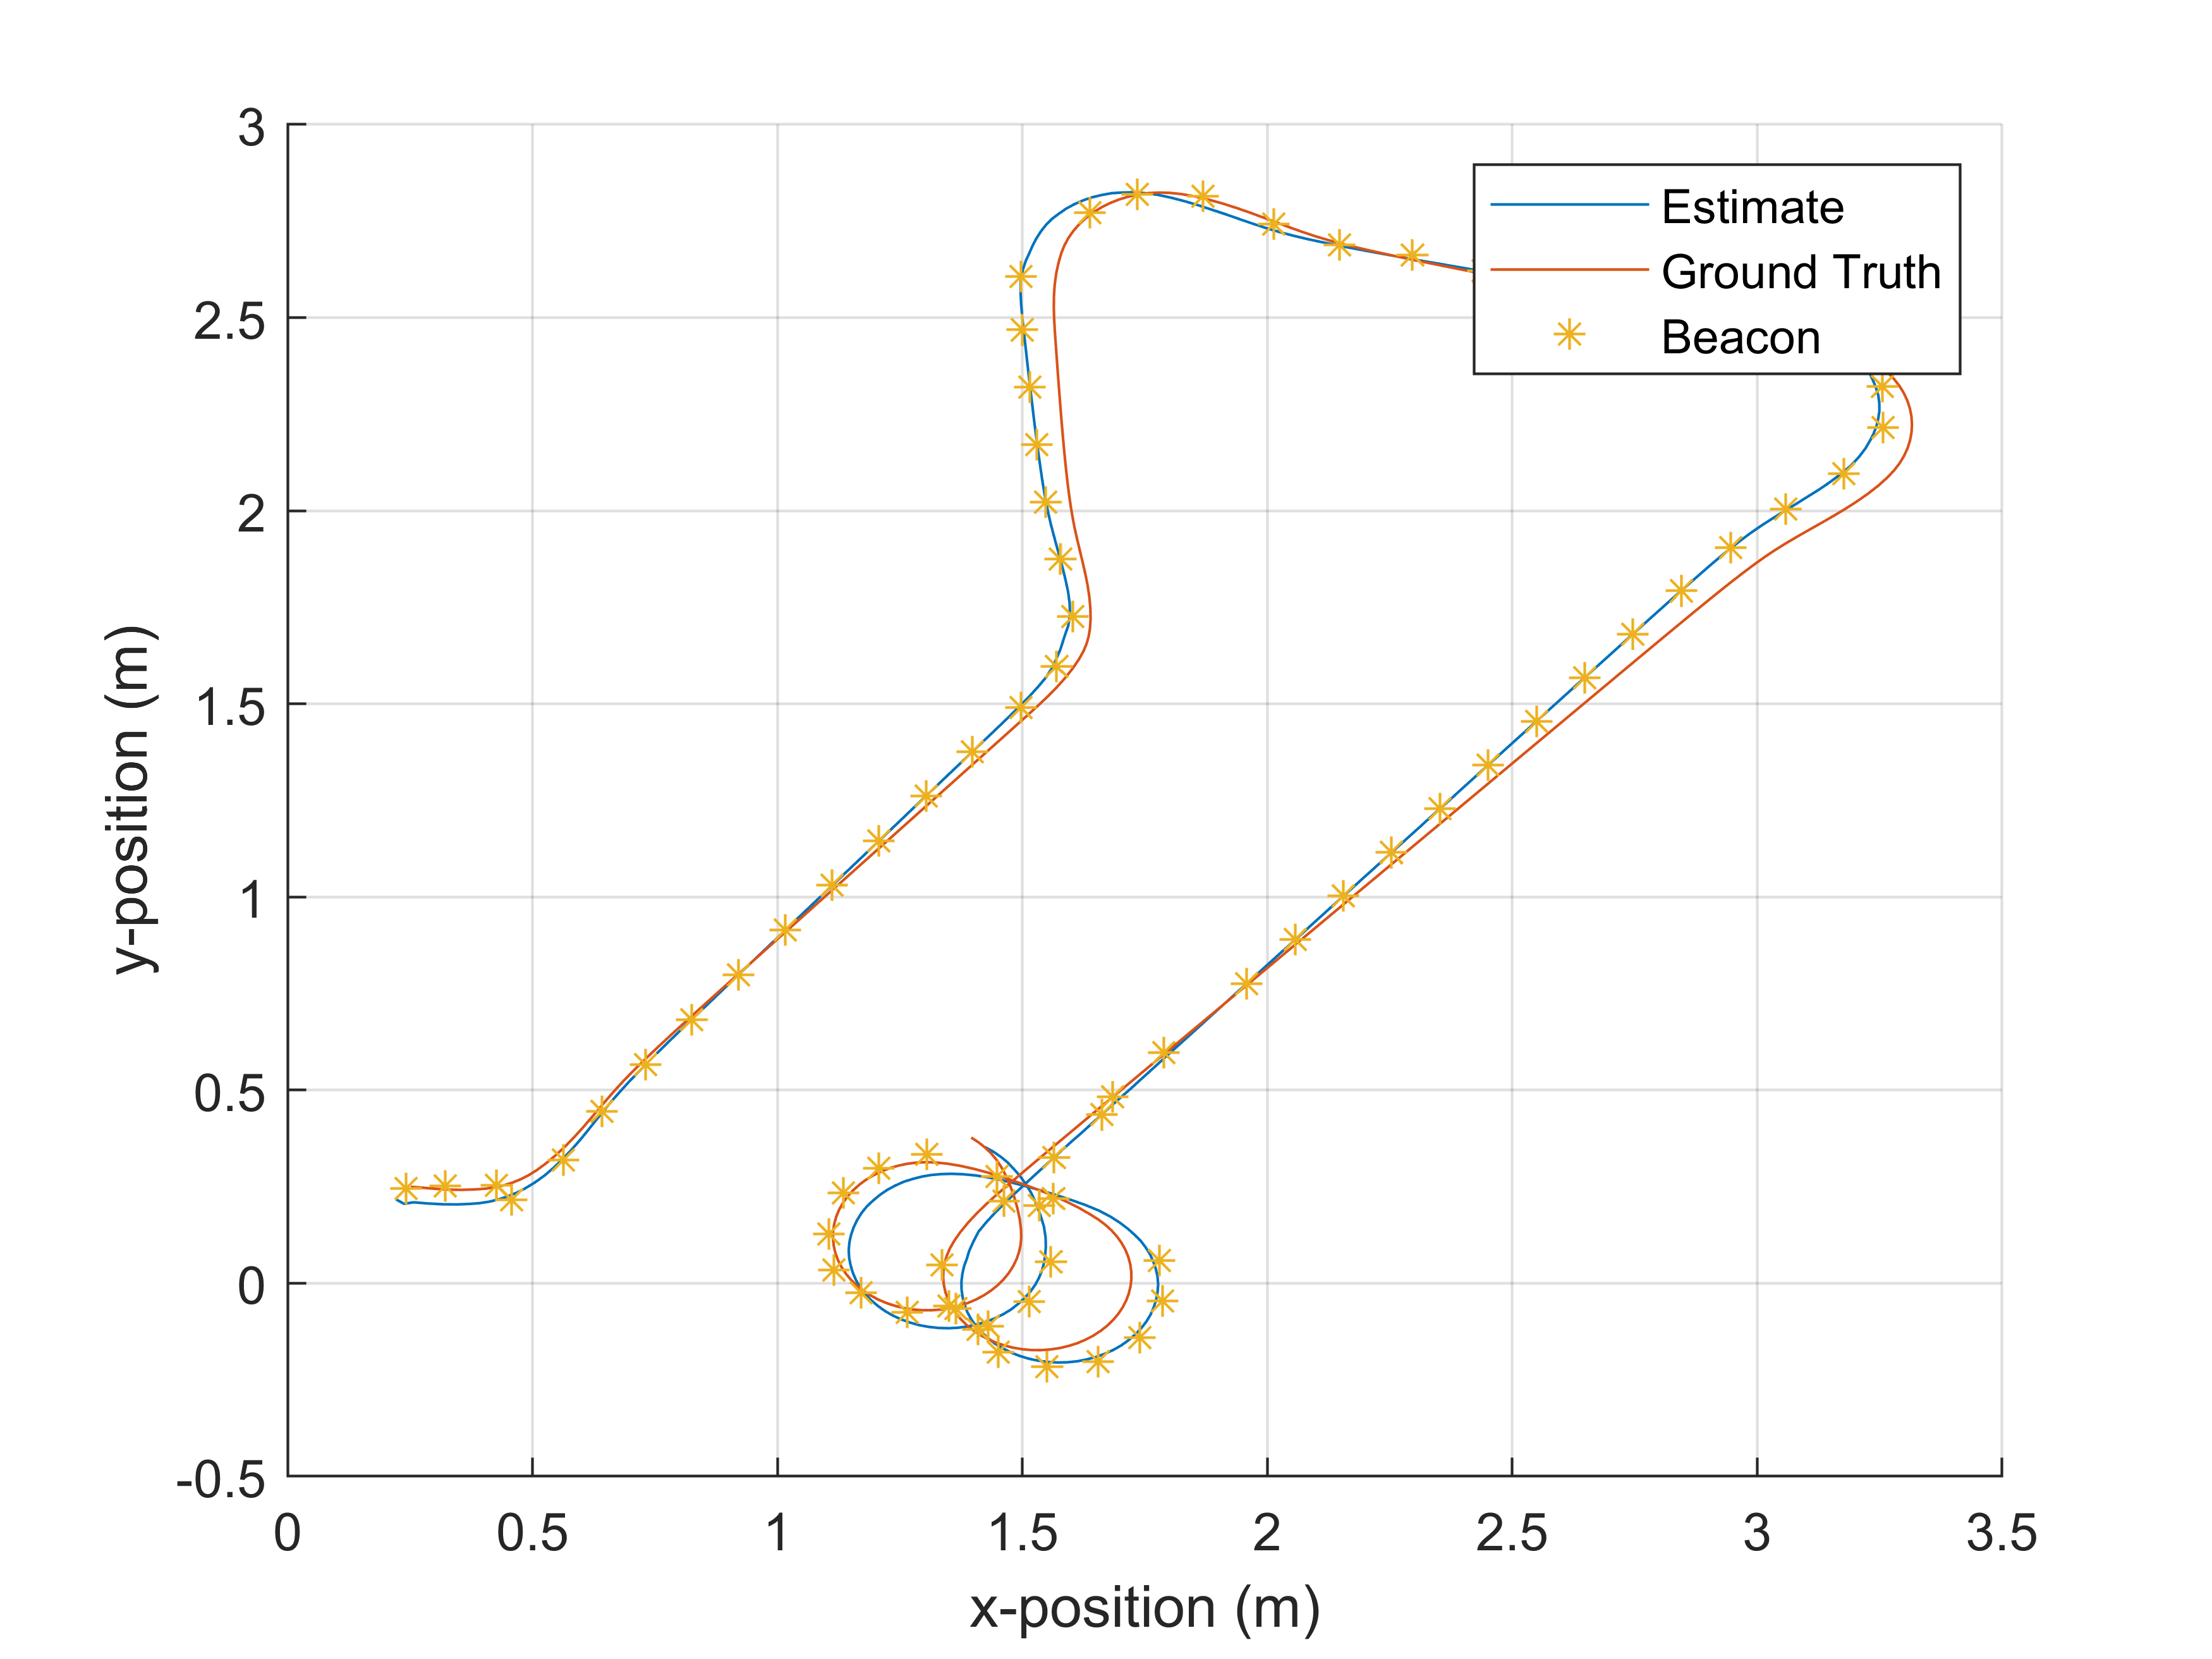
\includegraphics[width=\columnwidth]{./graphics/posSimu.png}
	   	\caption{Position estimates versus ground truth (Simulation).}
		\label{fig:pos}
	\end{figure}
	
	\begin{figure}
	    	\captionsetup{width=\columnwidth}
	   	\centering
	   	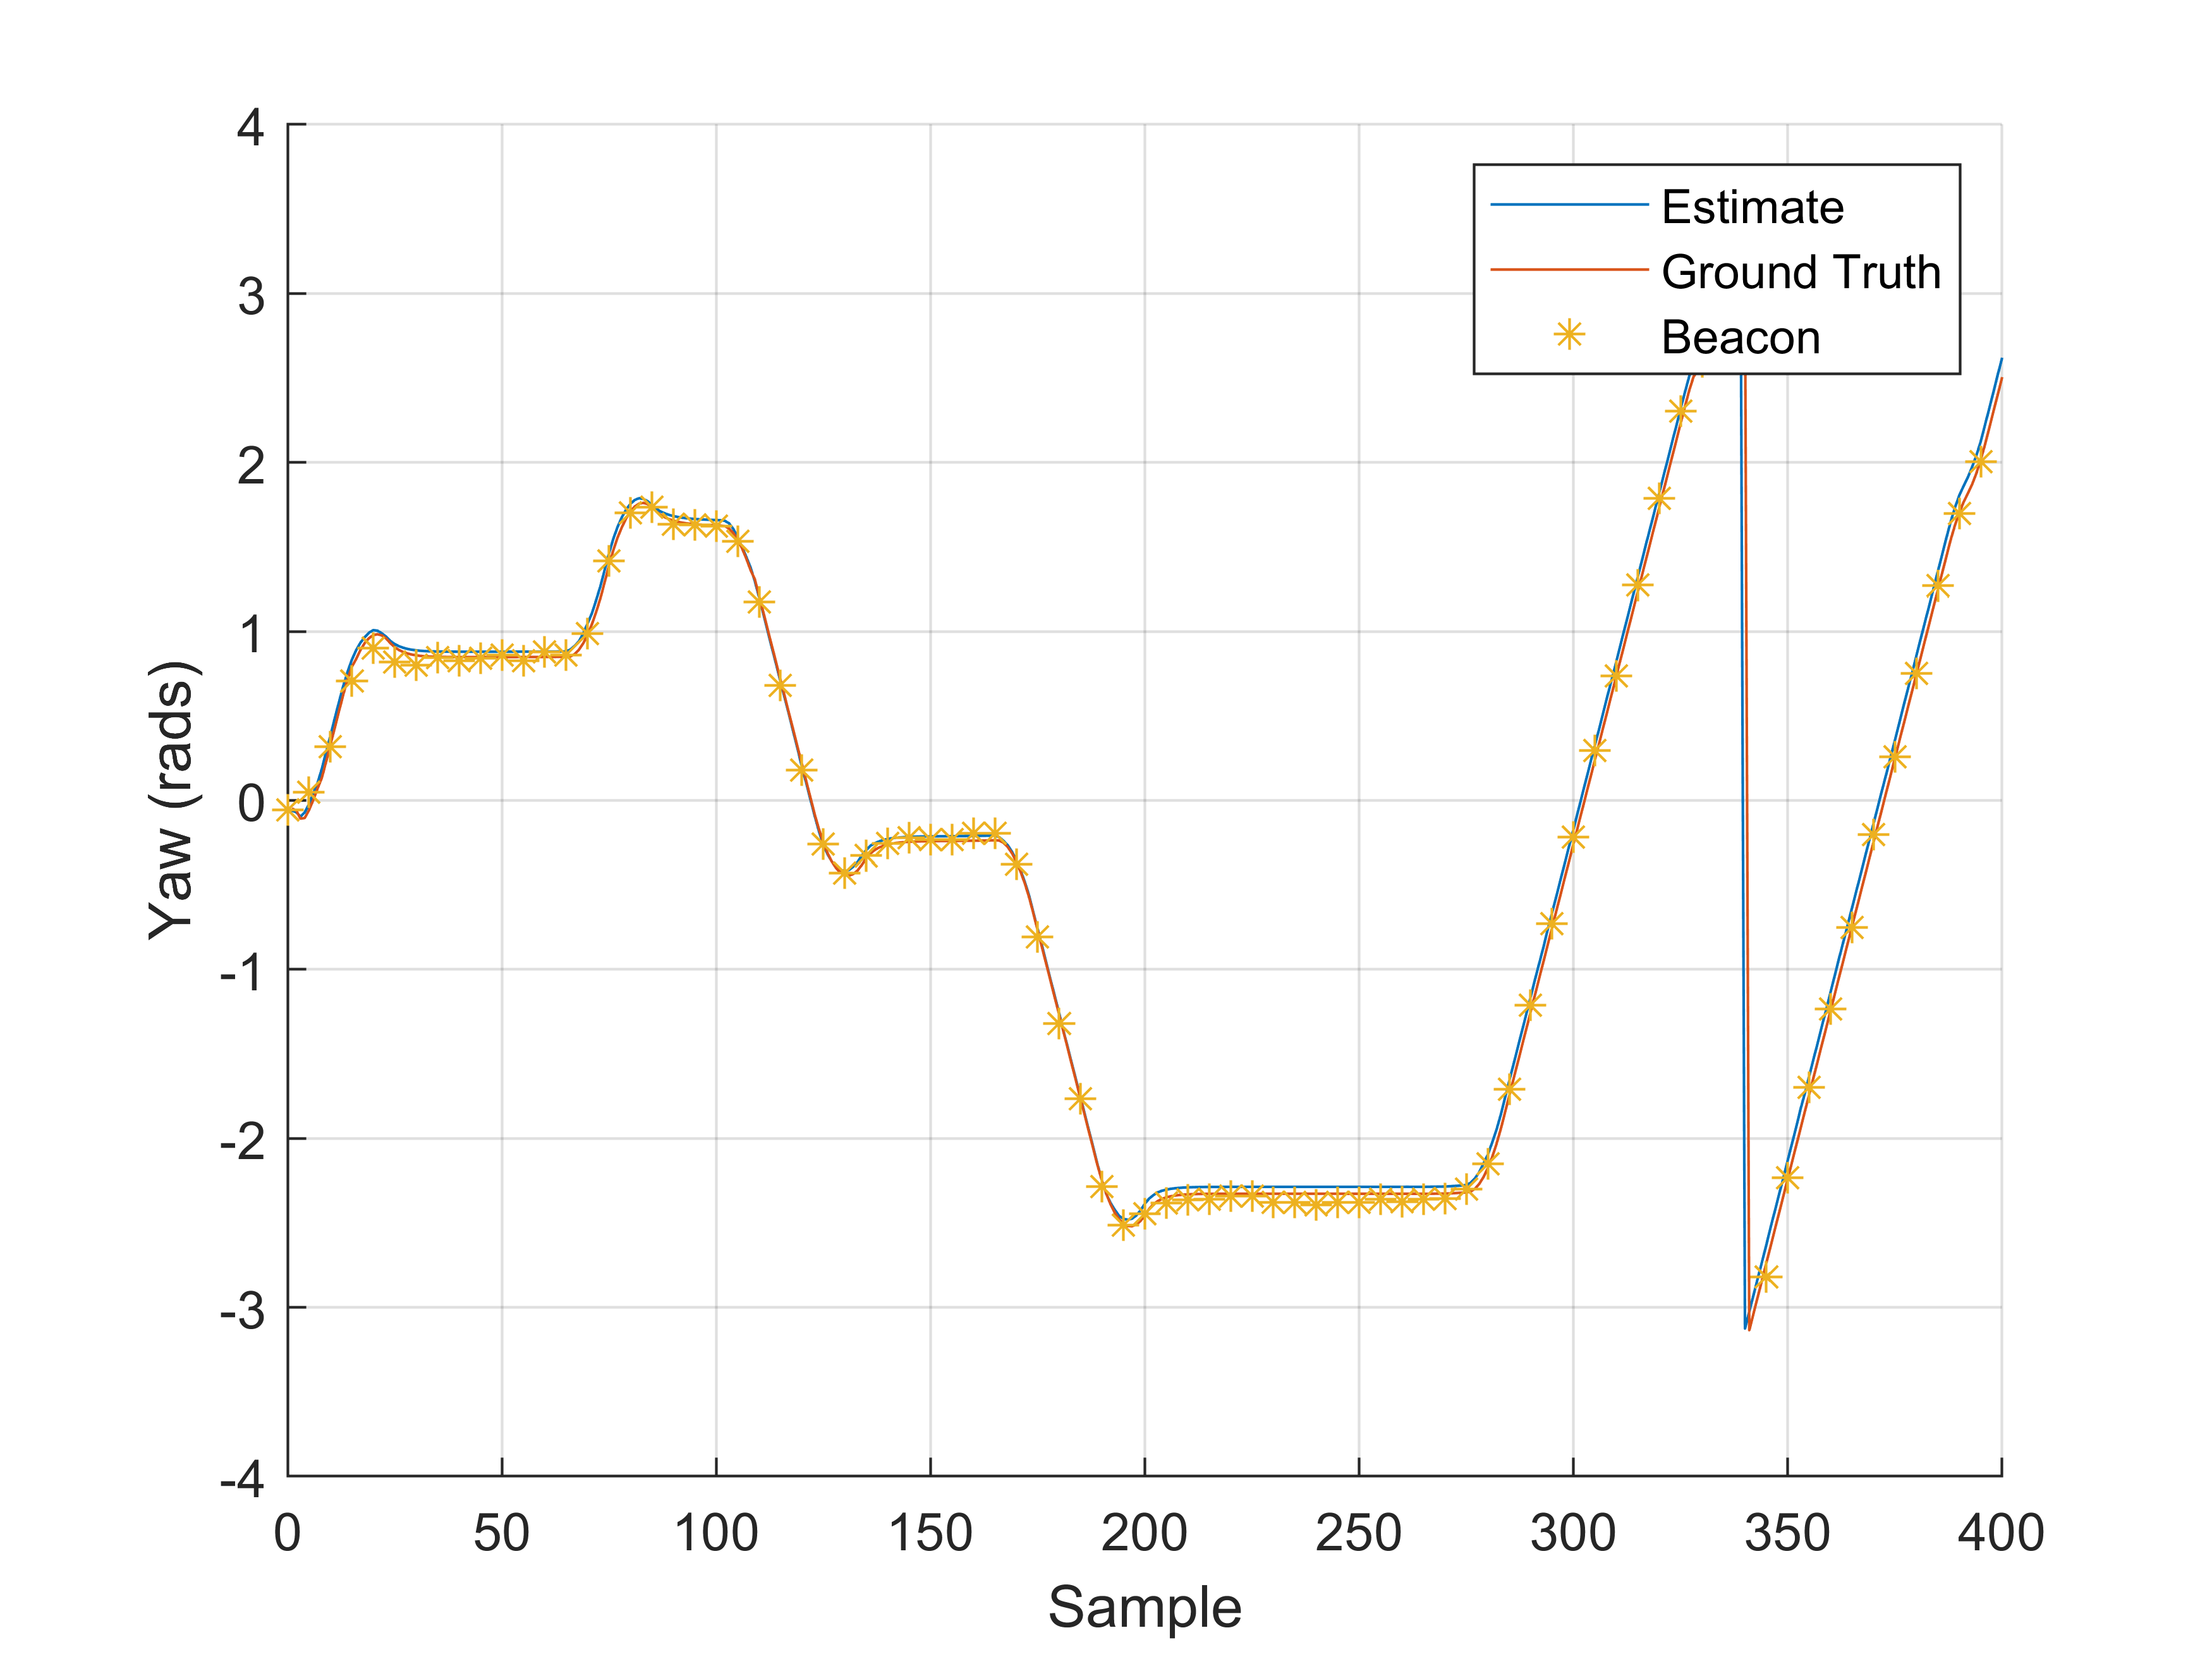
\includegraphics[width=\columnwidth]{./graphics/yawSimu.png}
	   	\caption{Yaw estimates versus ground truth (Simulation.}
		\label{fig:yaw}
	\end{figure}
	
	\begin{figure}
	    	\captionsetup{width=\columnwidth}
	   	\centering
	   	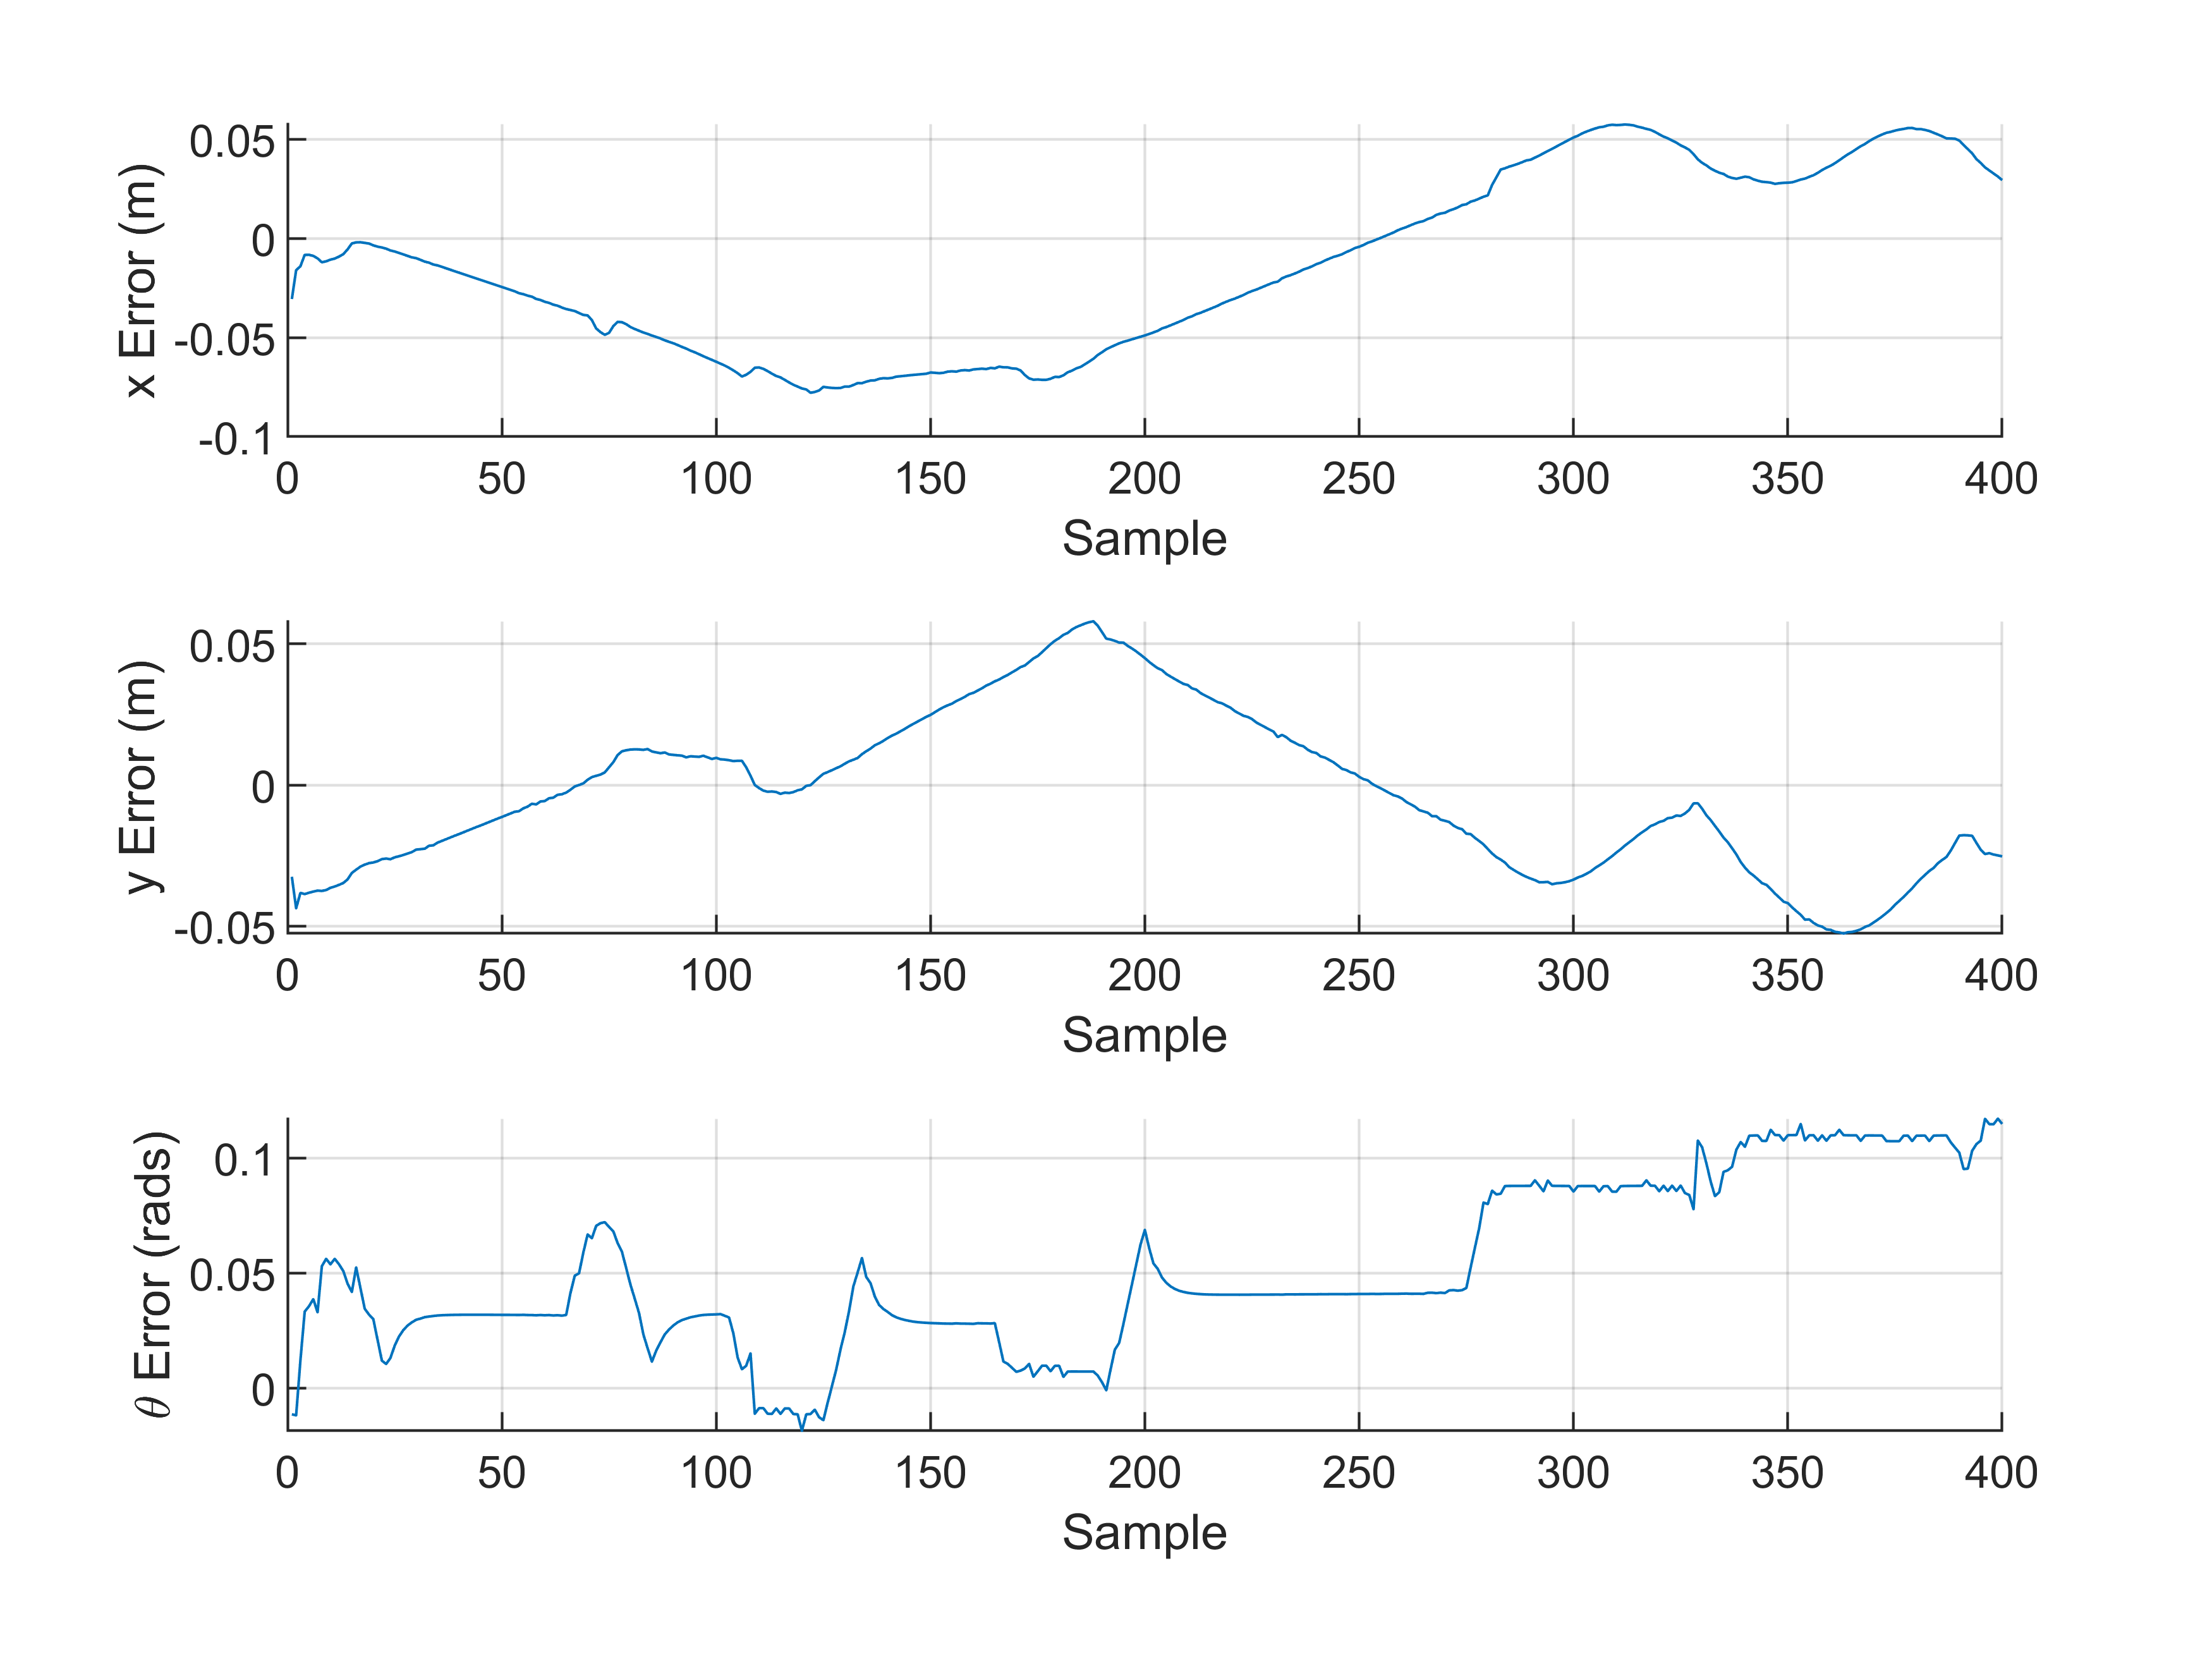
\includegraphics[width=\columnwidth]{./graphics/Error.png}
	   	\caption{Error plot of figure \ref{fig:pos} and \ref{fig:way}.}
		\label{fig:err2}
	\end{figure}